% $Header: /cvsroot/latex-beamer/latex-beamer/solutions/generic-talks/generic-ornate-15min-45min.en.tex,v 1.5 2007/01/28 20:48:23 tantau Exp $

\documentclass[12pt]{beamer}
%\documentclass[12pt,handout]{beamer}

% This file is a solution template for:

% - Giving a talk on some subject.
% - The talk is between 15min and 45min long.
% - Style is ornate.



% Copyright 2004 by Till Tantau <tantau@users.sourceforge.net>.
%
% In principle, this file can be redistributed and/or modified under
% the terms of the GNU Public License, version 2.
%
% However, this file is supposed to be a template to be modified
% for your own needs. For this reason, if you use this file as a
% template and not specifically distribute it as part of a another
% package/program, I grant the extra permission to freely copy and
% modify this file as you see fit and even to delete this copyright
% notice.


\mode<presentation>
{
  \usetheme{default}
  % or ...

  \setbeamercovered{transparent}
  % or whatever (possibly just delete it)
}
\setbeamertemplate{navigation symbols}{}%remove navigation symbols


\usepackage[english]{babel}
% or whatever

\usepackage[latin1]{inputenc}
% or whatever

\usepackage{times}
\usepackage{sansmathfonts}
\usepackage[T1]{fontenc}
% Or whatever. Note that the encoding and the font should match. If T1
% does not look nice, try deleting the line with the fontenc.


\title%[Short Paper Title] % (optional, use only with long paper titles)
{}

\subtitle
{} % (optional)

\author%[Author, Another] (optional, use only with lots of authors)
{Ben Holder}%{F.~Author\inst{1} \and S.~Another\inst{2}}
% - Use the \inst{?} command only if the authors have different
%   affiliation.

%\institute[Universities of Somewhere and Elsewhere] % (optional, but mostly needed)
%{
%  \inst{1}%
%  Department of Computer Science\\
%  University of Somewhere
%  \and
%  \inst{2}%
%  Department of Theoretical Philosophy\\
%  University of Elsewhere}
%% - Use the \inst command only if there are several affiliations.
%% - Keep it simple, no one is interested in your street address.

\date%[Short Occasion] % (optional)
{}

\subject{Talks}
% This is only inserted into the PDF information catalog. Can be left
% out.



% If you have a file called "university-logo-filename.xxx", where xxx
% is a graphic format that can be processed by latex or pdflatex,
% resp., then you can add a logo as follows:

% \pgfdeclareimage[height=0.5cm]{university-logo}{university-logo-filename}
% \logo{\pgfuseimage{university-logo}}



% Delete this, if you do not want the table of contents to pop up at
% the beginning of each subsection:
%\AtBeginSubsection[]
%{
%  \begin{frame}<beamer>{Outline}
%    \tableofcontents[currentsection,currentsubsection]
%  \end{frame}
%}


% If you wish to uncover everything in a step-wise fashion, uncomment
% the following command:

%\beamerdefaultoverlayspecification{<+->}

\usepackage{enumerate}
\usepackage{amsmath}
\usepackage{amssymb}
\usepackage[amssymb]{SIunits}
\usepackage{url}
\usepackage{hyperref}
\usepackage[normalem]{ulem}


\setbeamercovered{invisible}

\hypersetup{
    colorlinks=true,     % false: boxed links; true: colored links
    linkcolor=red,       % color of internal links
    citecolor=blue,      % color of links to bibliography
    filecolor=blue,      % color of file links
    urlcolor=blue        % color of external links
}


\begin{document}

%\begin{frame}
%  \titlepage
%\end{frame}

%%%%%%%%%%%%%%%%%%%%%%%%%%%%%%%%%%%%%%
\begin{frame}{Announcements}
	%
	\begin{itemize}
	\addtolength{\itemsep}{0.5\baselineskip}
	\item Any questions/issues?
	\item \underline{Schedule}:
		%
		\begin{itemize}
		\item[]{\bf Today (New)}: Oceans and Ice 
			%
			\begin{itemize}
			\item \underline{Physics}: coriolis,  buoyancy, thermal expansion
			\item \underline{Climate/Weather}: atmospheric and ocean currents, ENSO, Iceberg vs glacier melt, sea level
			\end{itemize}
			%
		\item[]{\bf Next Week (Wed Lab)}: Oceans and Ice
		\item[] {\bf Next Week (Tues/Thurs)}: Project Work.\\This is the last lecture!
		\end{itemize}
		%
	\end{itemize}

\end{frame}
%%%%%%%%%%%%%%%%%%%%%%%%%%%%%%%%%%%%%%
\begin{frame}{Today's Reading Quiz (3 min)}


%	
%\vspace{1cm}
%
%On your own sheet of paper\ldots
%
%\vspace{0.5cm}
%
%{\bf Briefly explain \underline{radiative forcing}. What are its units and why?  How does it affect temperature of the Earth? Can you give one example?}
%\vspace{0.5cm}
%
%Turn in to Blackboard as scanned pdf (or image is fine).


No reading for today, but find additional resources for these topics in:
	%
	\begin{itemize}
	\item {\em Mathez}: Chap 3 --- Ocean-Atmos Interactions (El Ni\~no)
	\item {\em My notes}: Fluid statics (Buoyant Force, Floating) 
	\end{itemize}
	%
both of which can be found on Blackboard under ``Class Lecture Slides''
	

\end{frame}
%%%%%%%%%%%%%%%%%%%%%%%%%%%%%%%%%%%%%%
\begin{frame}{Final Poster Project}

\begin{itemize}
\item Choose a topic that is interesting to you and make a poster to present (5min) to the class during our final exam period (Thurs, Dec 11, 10am--Noon).
\item Work on your own or with a partner.
\item Think of it as a Discussion/Lab/Lecture that you create, explaining some topic to yourself and us.
\item {\bf Talk to me by Thanksgiving (Tues Nov 25)} to verify your project topic ({\bf that chat is worth one Discussion assignment}).
\item In the last week of class you will have time (lecture and discussion) to work on your final poster project. 
	
\end{itemize}


\end{frame}
%%%%%%%%%%%%%%%%%%%%%%%%%%%%%%%%%%%%%%
\begin{frame}{Newton's Laws and ``Fictitious'' Forces}

\begin{itemize}
\item Recall that Newton's Second Law tells us:
	%
	\begin{equation*}
	\sum \vec{F} = m \, \vec{a}
	\end{equation*}
	%
An object will {\em accelerate} (change its velocity vector) due to the sum of the forces acting on it.

\item  We say a force is ``fictitious'' if an object accelerates without any force to explain it.
\end{itemize}

\vspace{5cm}


\end{frame}
%%%%%%%%%%%%%%%%%%%%%%%%%%%%%%%%%%%%%%
\begin{frame}{Coriolis Effect}

\begin{itemize}
\item The circulation of the atmosphere is due to fictitious forces arising from the rotation of the Earth.  These are called {\bf Coriolis} forces, or the ``coriolis effect.''
\item We can understand these dynamics by first \href{https://www.youtube.com/watch?v=mPsLanVS1Q8}{investigating the playground ``merry-go-round'' ride}.
\end{itemize}

\begin{center}
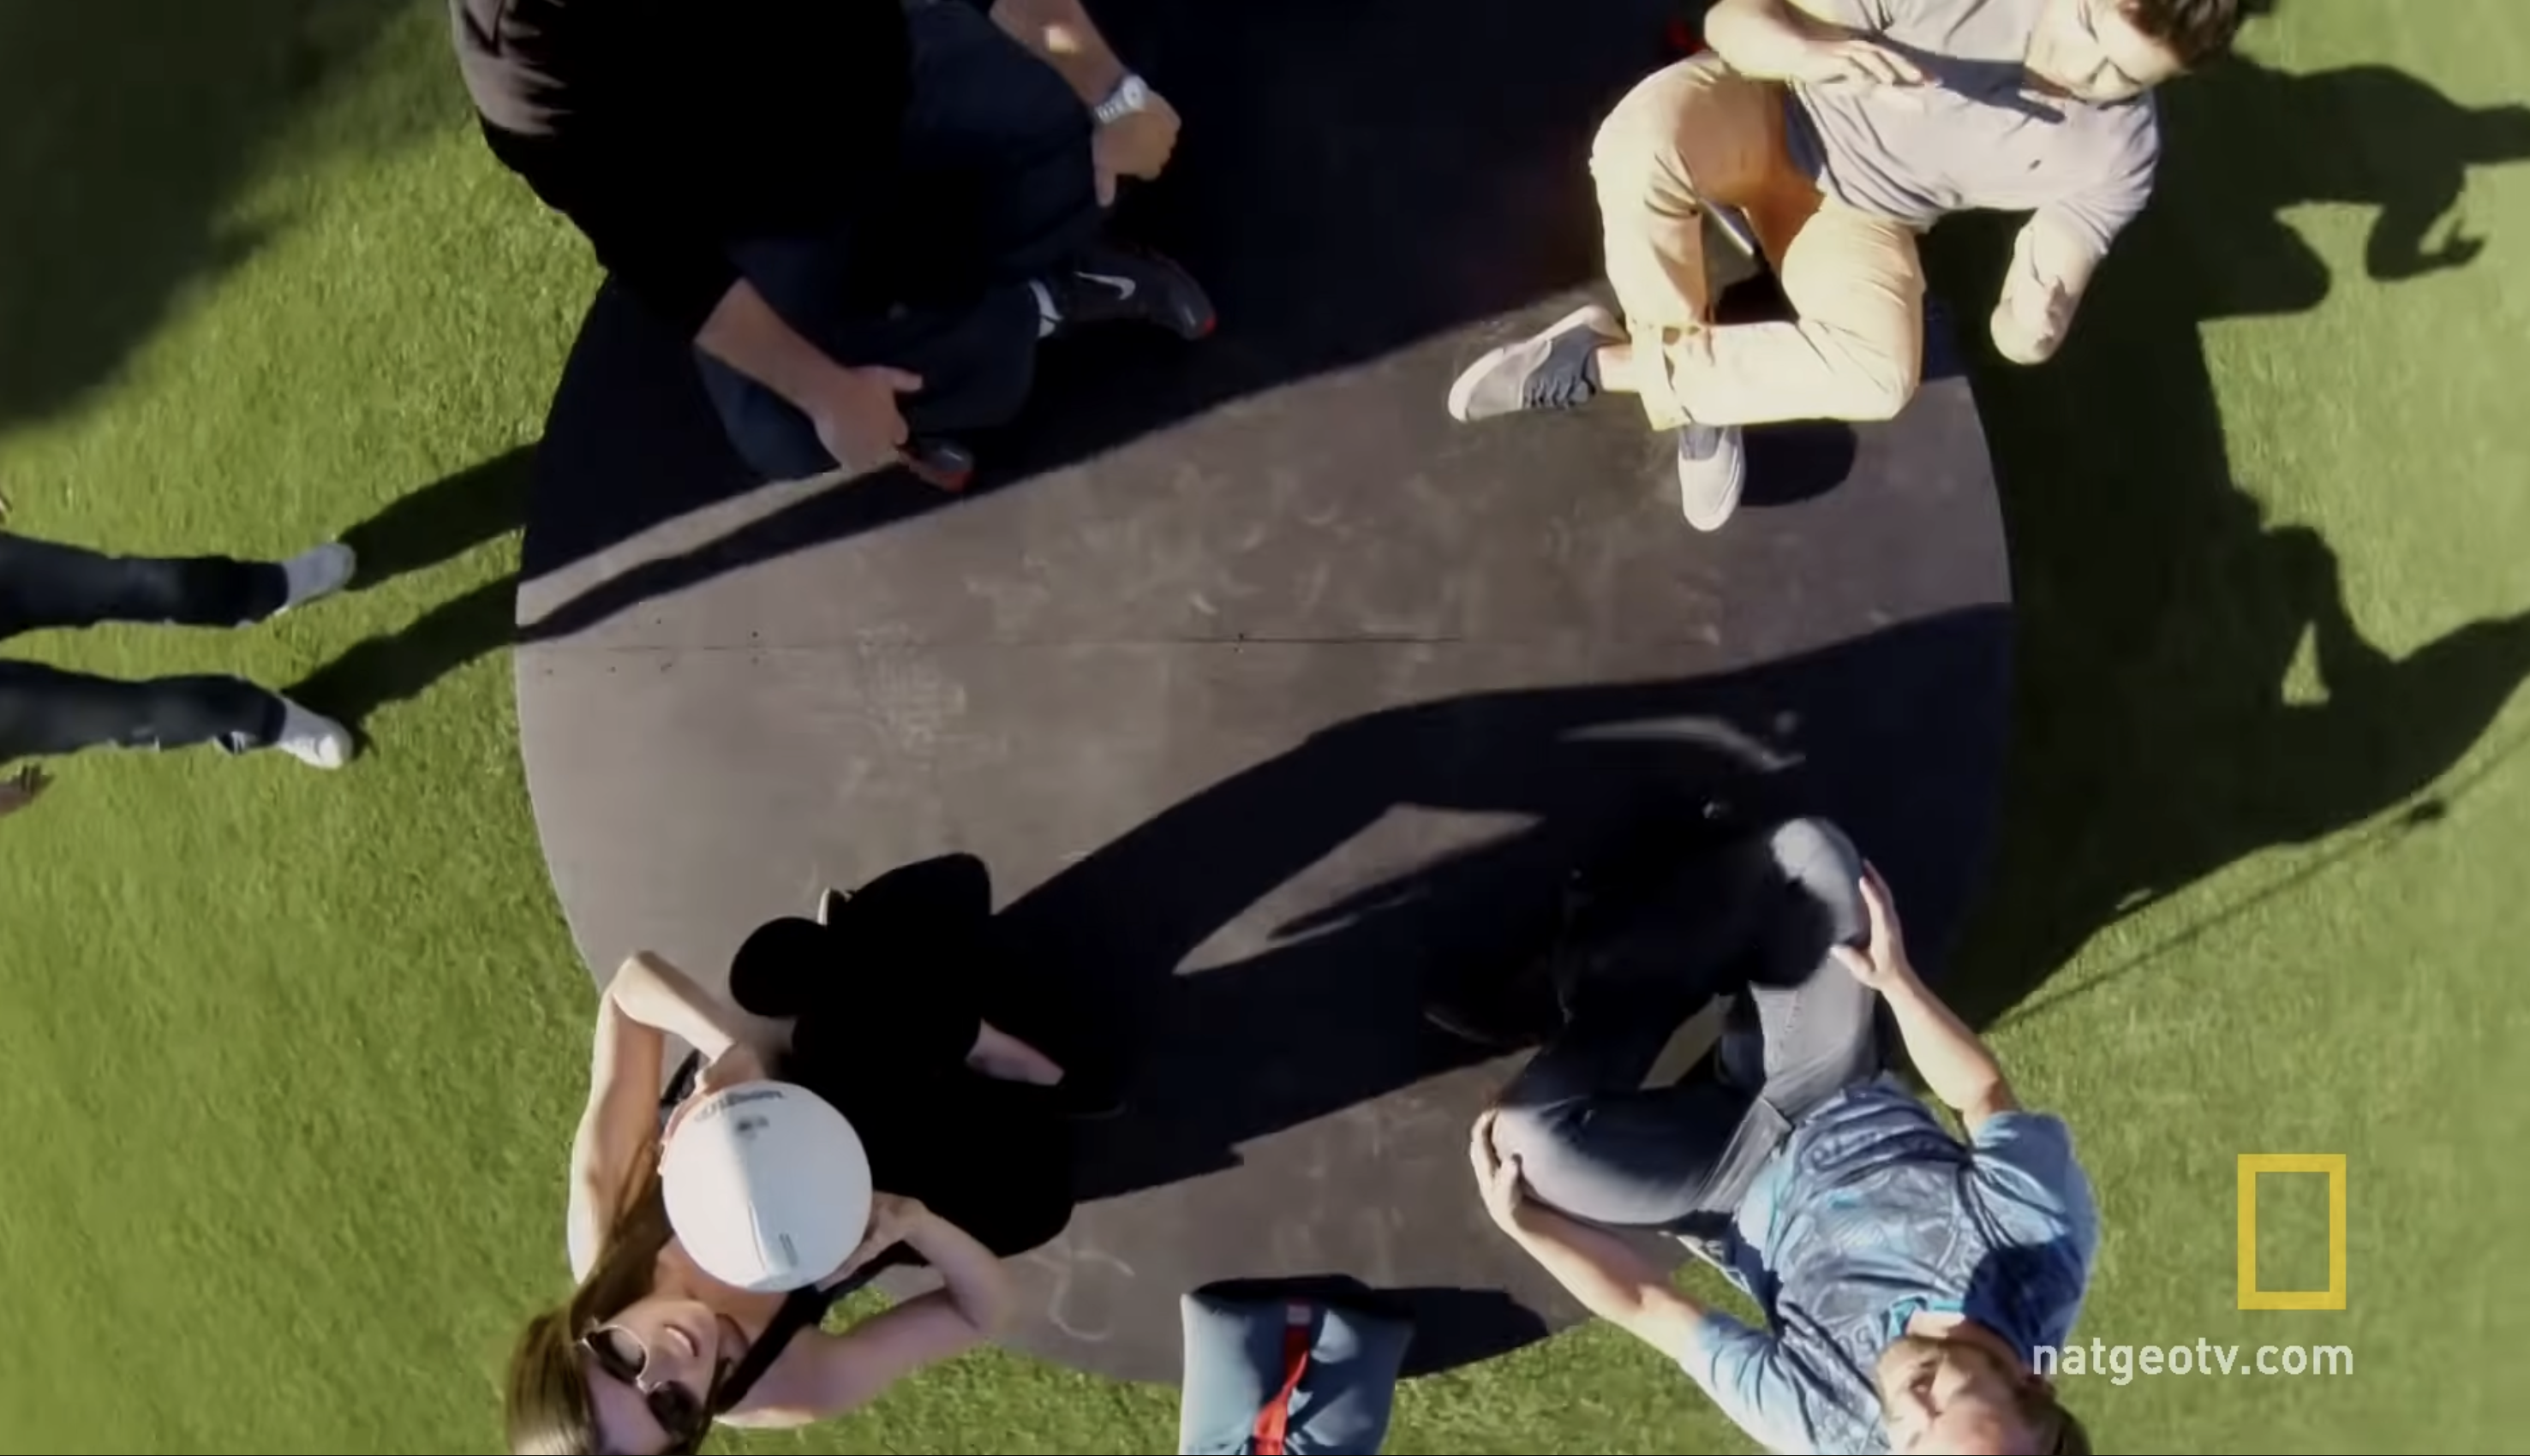
\includegraphics[width=0.8\textwidth]{images/merry-go-round-nat-geo}
\end{center}

\begin{itemize}
\item Net result: in the Northern Hemisphere flows ``turn right''.
\end{itemize}


\end{frame}
%%%%%%%%%%%%%%%%%%%%%%%%%%%%%%%%%%%%%%
\begin{frame}{Coriolis Effect and Trade Winds}

\begin{itemize}
\item Let's try to understand the origin of the ``trade winds,'' that flow from East to West along the equator.
\end{itemize}

\vspace{6cm}


\end{frame}
%%%%%%%%%%%%%%%%%%%%%%%%%%%%%%%%%%%%%%
\begin{frame}{El Ni\~no, La Ni\~na, and ENSO}


\begin{center}
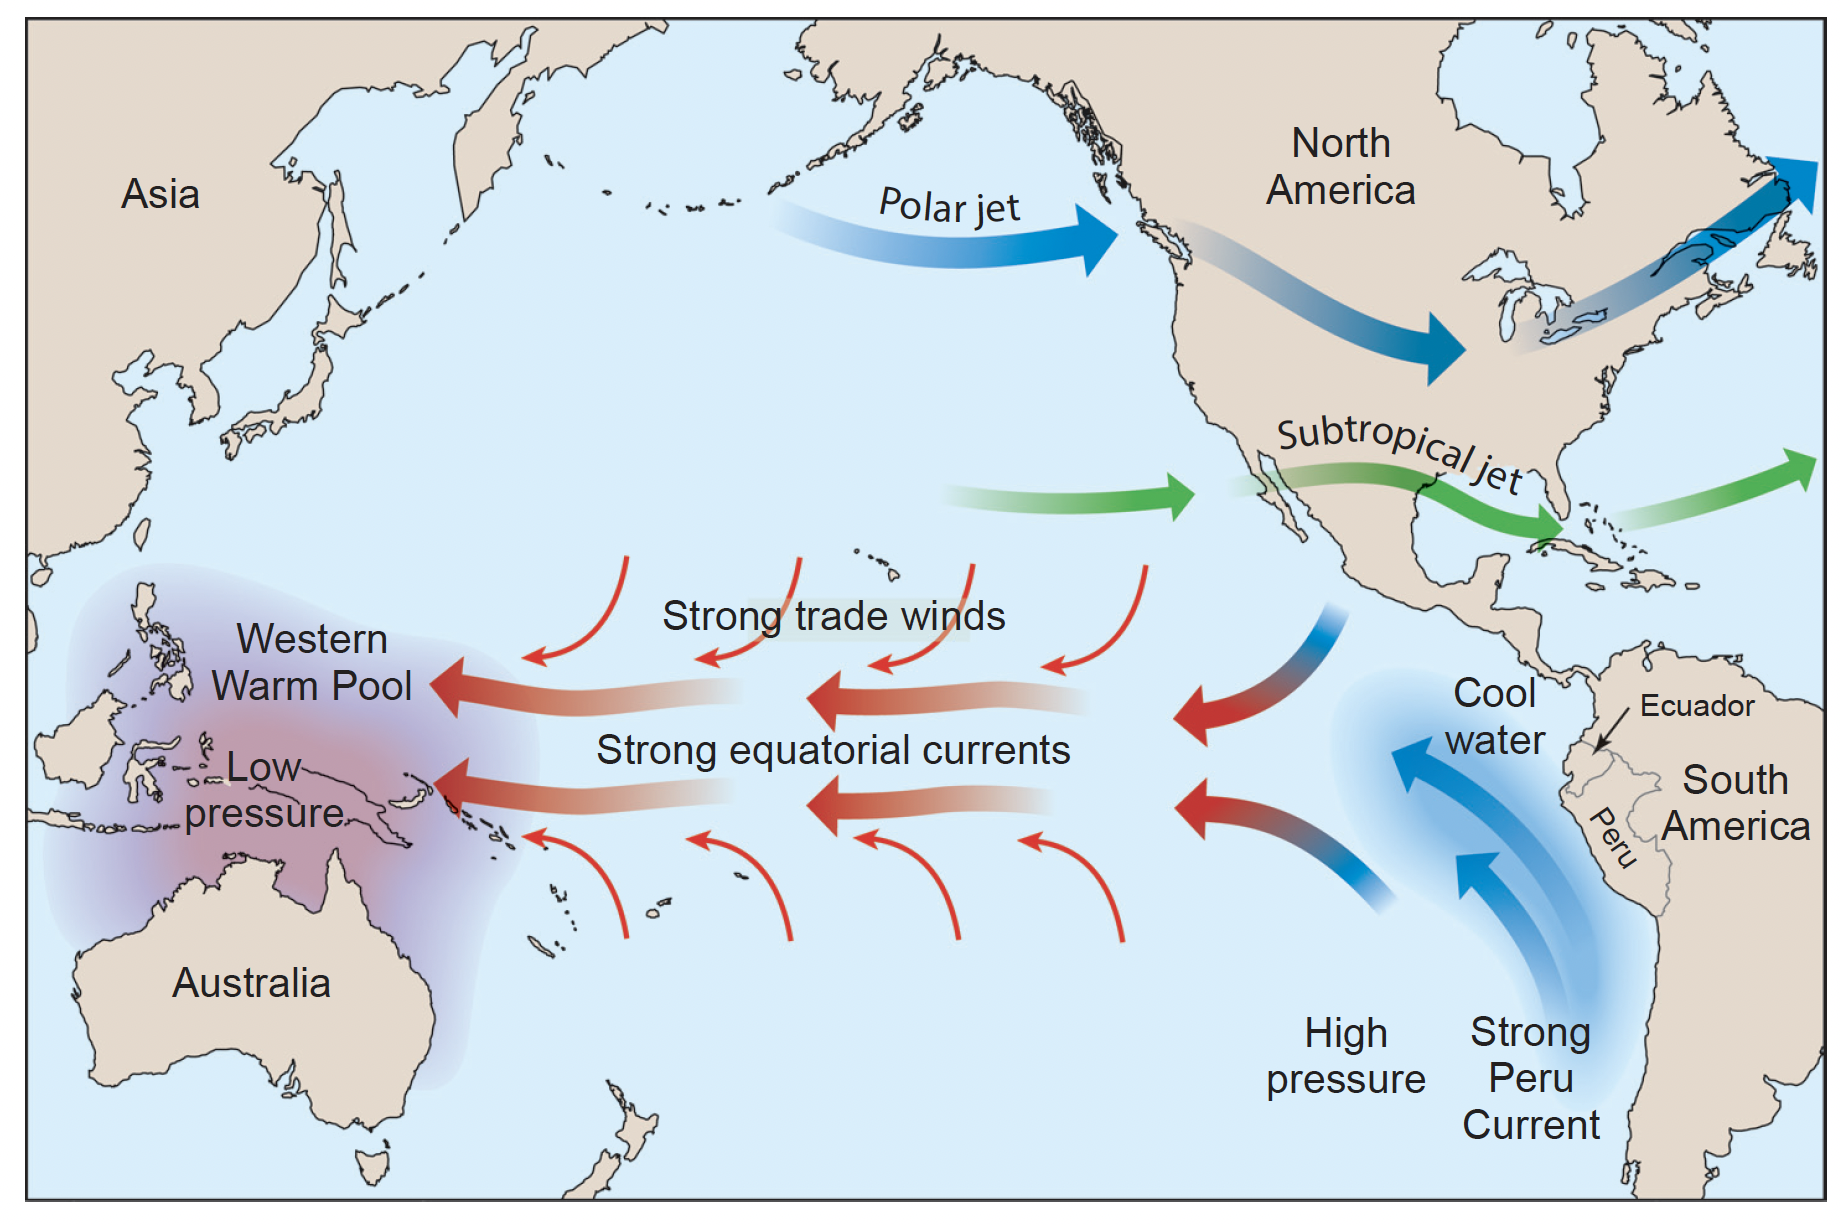
\includegraphics[width=\textwidth]{images/mathez_fig3-1_neutral-state.png}\\
{\tiny \bf {\em Mathez} Figure 3.1: The neutral state of the tropical Pacific Ocean}
\end{center}


\end{frame}
%%%%%%%%%%%%%%%%%%%%%%%%%%%%%%%%%%%%%%
\begin{frame}{El Ni\~no, La Ni\~na, and ENSO}


\begin{center}
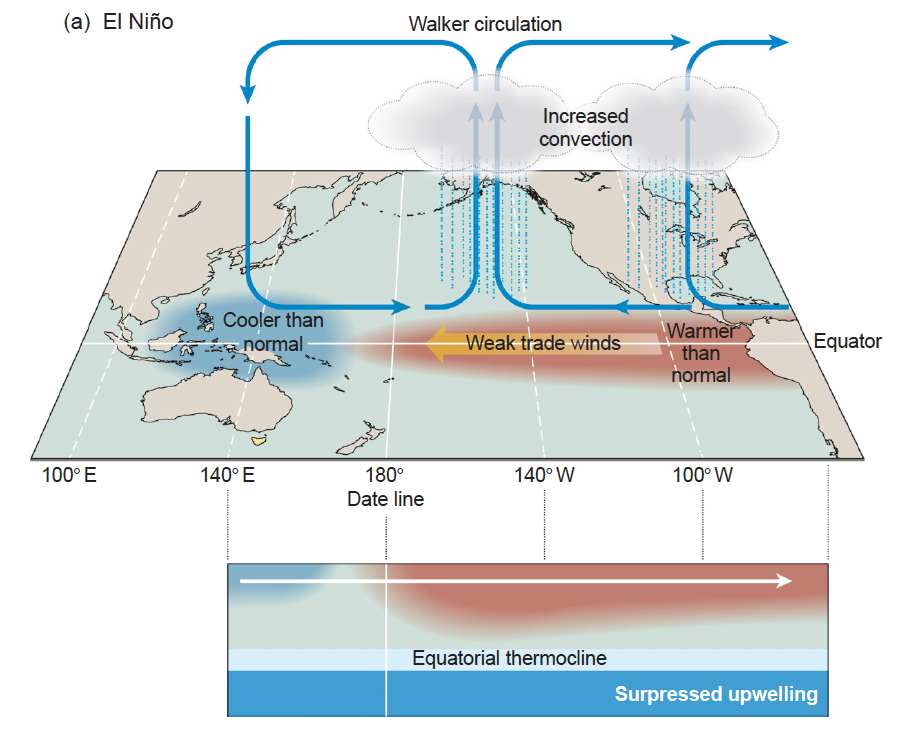
\includegraphics[width=0.48\textwidth]{images/mathez_fig3-4_el-nino-la-nina-I.png}  \hfill %
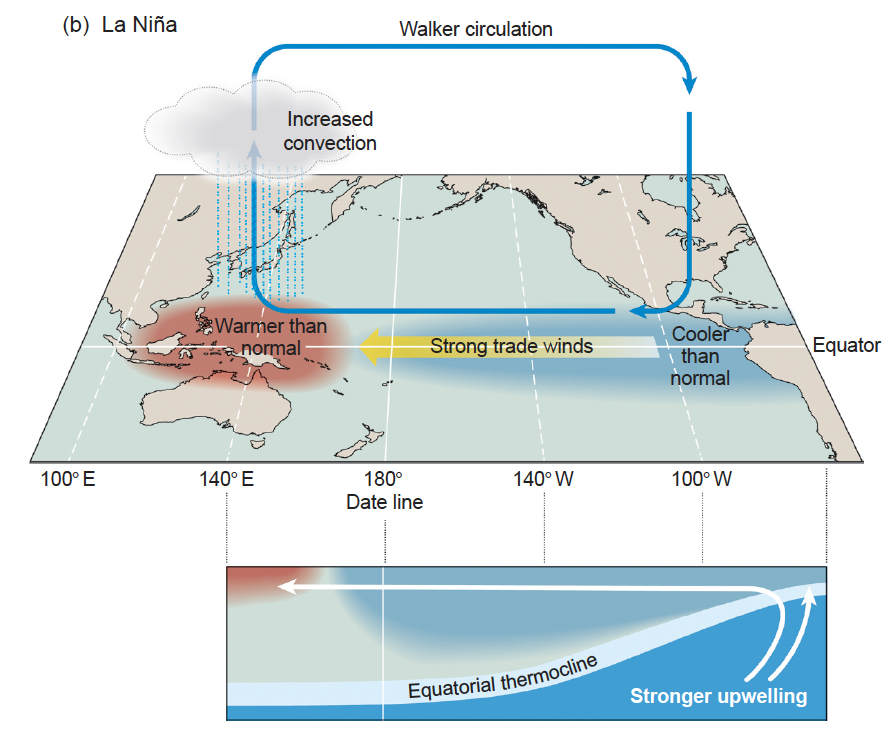
\includegraphics[width=0.48\textwidth]{images/mathez_fig3-4_el-nino-la-nina-II.png} 
{\tiny \bf {\em Mathez} Figure 3.4}
\end{center}


\end{frame}
%%%%%%%%%%%%%%%%%%%%%%%%%%%%%%%%%%%%%%
\begin{frame}{El Ni\~no, La Ni\~na, and ENSO}


\begin{center}
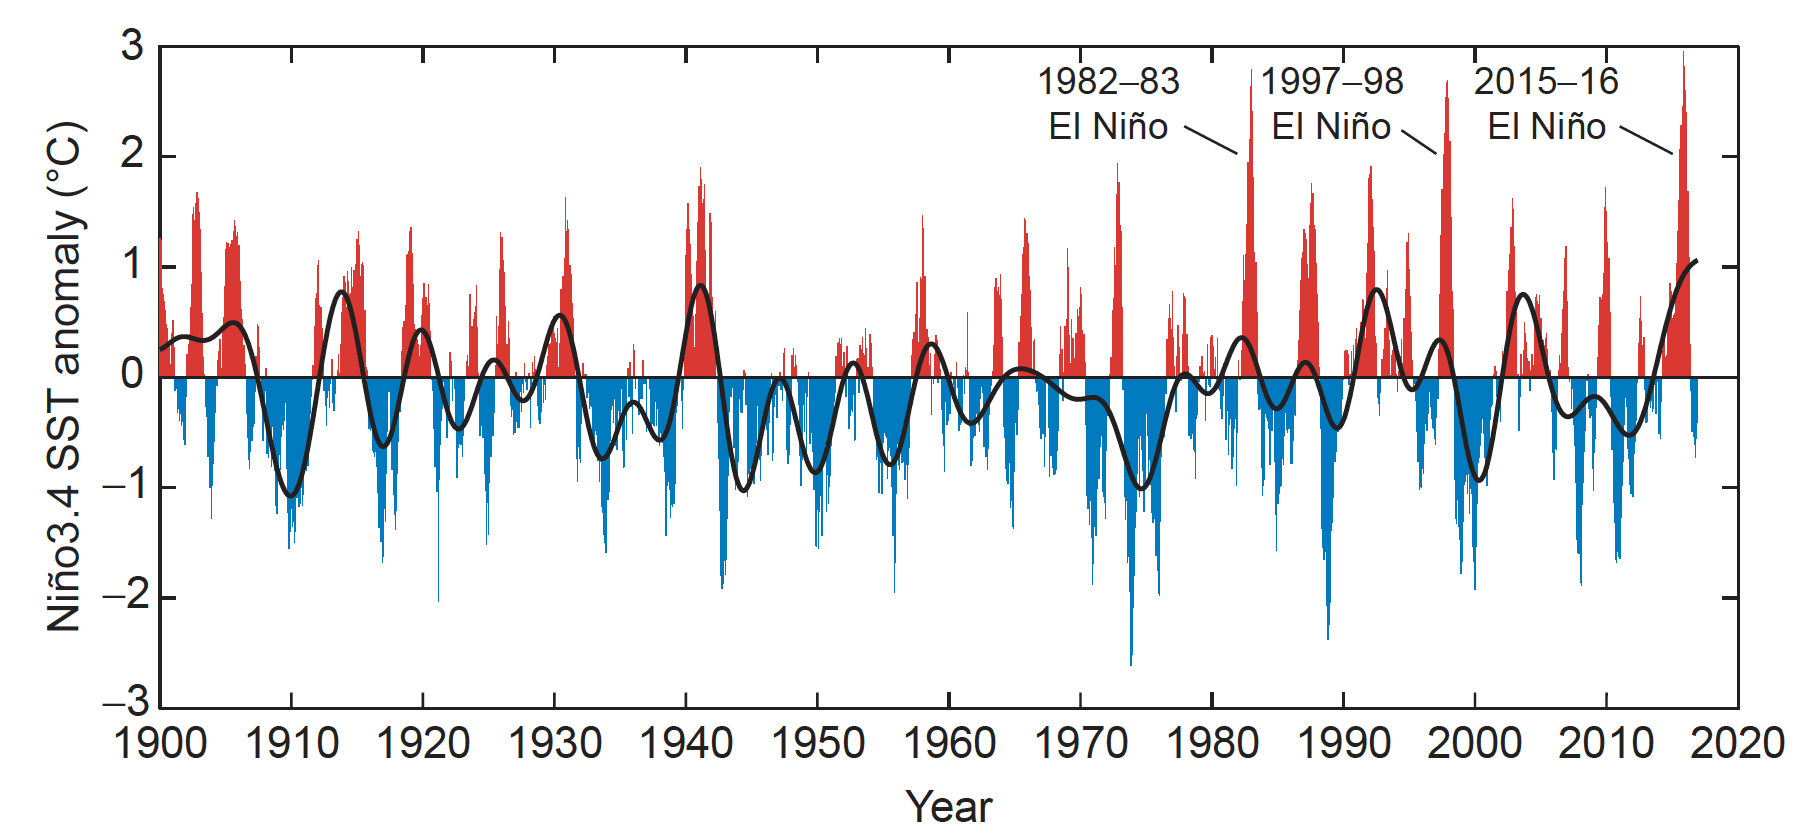
\includegraphics[width=\textwidth]{images/mathez_fig3-5_nino-events.png}\\
{\tiny \bf {\em Mathez} Figure 3.5}
\end{center}


\end{frame}
%%%%%%%%%%%%%%%%%%%%%%%%%%%%%%%%%%%%%%
\begin{frame}{ENSO and Global Temperature}


\begin{center}
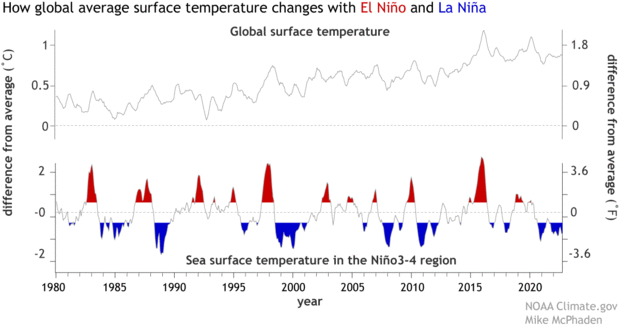
\includegraphics[width=\textwidth]{images/global-temp-nino_climate-gov.png}\\
{\tiny \href{https://www.climate.gov/news-features/blogs/enso/where-does-global-warming-go-during-la-nina}{Climate.gov}}
\end{center}


\end{frame}
%%%%%%%%%%%%%%%%%%%%%%%%%%%%%%%%%%%%%%
\begin{frame}{Buoyant Force, Floating, Ice}

\begin{itemize}
\item We define the {\bf buoyant force} on an object within a fluid as the sum of the pressure forces that it experiences.
\item Since the displaced fluid is exactly held in equilibrium, the buoyant force is:
	%\
	\begin{equation*}
	F_B = \text{weight of fluid displaced}
	\end{equation*}
\item We can use this to understand which objects float, and how much they are submerged.
\end{itemize}


\end{frame}
%%%%%%%%%%%%%%%%%%%%%%%%%%%%%%%%%%%%%%



\end{document}
